% Metódy inžinierskej práce

\documentclass[10pt,twoside,a4paper]{article}
\usepackage[]{babel}
%\usepackage[T1]{fontenc}
\usepackage[]{fontenc} % lepšia sadzba písmena Ľ než v T1
\usepackage[utf8]{inputenc}
\usepackage{graphicx}
\usepackage{url} % príkaz \url na formátovanie URL
\usepackage{hyperref} % odkazy v texte budú aktívne (pri niektorých triedach dokumentov spôsobuje posun textu)


\usepackage{cite}
%\usepackage{times}

\pagestyle{headings}

\title{Rozšírená realita a jej využitie v každodennom živote\thanks{Semestrálny projekt v predmete Metódy inžinierskej práce, ak. rok 2022/23, vedenie: Igor Stupavský}} % meno a priezvisko vyučujúceho na cvičeniach

\author{Martin Podmanický\\[2pt]
	{\small Slovenská technická univerzita v Bratislave}\\
	{\small Fakulta informatiky a informačných technológií}\\
	{\small \texttt{xpodmanickym@stuba.sk}}
	}

\date{\small 18. október 2022} % upravte



\begin{document}

\maketitle

\begin{abstract}
Tento článok je zameraný na fungovanie rozšírenej reality v bežnom a profesionálnom živote. Lepšie pochopenie ako nám môže dopomôcť k pochopeniu zložitých problémov a celkovému zlepšeniu ľudského myslenia. Rôzne príklady rozšírenej reality z nášho sveta v zdravotníctve, školstve, strojárstve. Využitie vážnych hier ako skutočnej pomôcky pri učení. Motiváciou je vysvetlenie a objasnenie rozšírenej reality v bežnom a profesionálnom živote, v rôznych odvetviach priemyslu a jej výhod ako aj pomoc pre študentov trpiacich poruchami sústredenia a ADHD, a ako im práve rozšírená realita dokáže uľahčiť každodenné povinnosti. Taktiež riešenie problémov v bežnom svete a svete hernom, a akú revolúciu by to mohlo priniesť medzi nás.
\ldots
\end{abstract}



\section{Úvod}
\par Rozšírená realita sa postupom času zdokonalila a začala sa využívať v rôznych odvetviach a častiach našich životov. Otvorila dvere mnohým novým možnostiam interakcie skutočného sveta s technológiami. Mnohý ľudia využívajú smartfóny a smart hodinky, ktoré sú niekedy v ceste, vyzerajú nespratné a niekedy nie sú až tak "smart". Práve preto by virtuálna realita spárovaná so správnym hardvérom mohla dominovať dobe smratfónov a dokonca ich úplne vyradiť. Využitie hardvéru vybaveného virtuálnou realitou by však nebolo využívané len na jednu konkrétnu vec ale na všetky tie, na ktoré treba smartfón. O hardvére sa rozprávame ako o optickom aparáte nejakého typu, ktorý by premietal všetky informácie, ktoré by užívateľ vyžadoval a potreboval. Zamerané je to všetko na povinnosti a riešenie problémov v bežnom živote.


Priblíženie a fungovanie Rozšírenej reality~\ref{co} a~\ref{ako}.
Jej využitie v momentálnej dobe~\ref{vyuzitie}.
Virtuálna realita a vážne hry~\ref{vz}.
Využitie v iných odvetviach~\ref{zdravotnictvo}.
Zhodnotenie a spätný pohľad prináša sekcia~\ref{konec}.
Záverečné poznámky prináša časť~\ref{zaver}.



\section{Čo to vlastne je} \label{co}

Rozšírená realita nie je nič zložité ani náročné na pochopenie. Ide v podstate o to, čomu názov nasvedčuje = rozširuje realitu. Rozširuje realitu o prvky, ktoré v skutočnosti nie sú fyzicky hmatateľné. Vrstva z digitálneho prostredia je tak implementovaná do našich životov a narozdiel od virtuálnej reality, ktorá vytvára aj umelé prostredie, nijak neprekáža v normálnom fungovaní života ba podľa všetkého by k tomu mala ešte dopomáhať a zefektívniť, aspoň teda vybrané zariadenia. V súčastnosti rozšírená realita vytvára  3D koncept, ktorý sa priamo premieta do prostredia. Najväčšie využitie je však v zábavnom priemysle.

\section{Ako to funguje}\label{ako}

Teraz keď už máme obraz o tom, čo to je, poďme zistiť ako to celé funguje. Používajú sa rôzne obsahy, konkrétnejšie obrázky, animácie, 3D modely alebo aj video, ktoré môžu byť zobrazované na iných zariadeniach  s obrazovkou. Mobilný telefón, displej a podobne. K fungovaniu rozšírenej reality, je za potreba senzorov. Cez fotoaparát a iné senzory na zariadení sa zhromažďujú informácie o užívateľovom okolí a jeho interakciách. \par Tieto informácie sa následne odosielajú na spracovanie. Nakoniec, na naskenované prostredie cez fotoaparát alebo kameru v zariadení, je možné umiestňovať do prostredia vygenerované modely. Práve toto bol obrovský úspech hry PokemonGO, ktorá využívala systém rozšírenej reality. K rozšírenej realite patrí však aj projekcia. Tak ako pracuje s prostredím a sníma okolie, dokáže doň cez projektory vkladať generované 3D modely. Predstavte si to ako hologramy z filmov ale také, s ktorými je možno narábať avšak nie sú hmotné.

Z obr.~\ref{f:rozhod} je všetko jasné. 

\begin{figure*}[tbh]
\centering
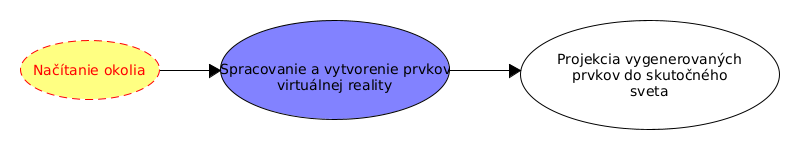
\includegraphics[scale=0.5]{Diagram fungovania AR.png}
%Aj text môže byť prezentovaný ako obrázok. Stane sa z neho označený plávajúci objekt. Po vytvorení diagramu zrušte znak \texttt{\%} pred príkazom \verb|\includegraphics| označte tento riadok ako komentár (tiež pomocou znaku \texttt{\%}).
\caption{Diagram rozšírenej reality a skutočného sveta.}
\label{f:rozhod}
\end{figure*}



\section{Ako ju vie využiť naša spoločnosť} \label{vyuzitie}
\subsection{Súčasnosť}\label{vyuzitie:suc}
\par V súčasnej dobe sa stretávame s rozšírenou realitou najmä na našich smartfónoch. Najznámejšie budú filtre z aplikácie Snapchat, ktoré nasnímajú vašu tvár a potom podľa vašej preferencie na ňu premietne model alebo obraz. Takisto v už aj spomínanej hre PokemonGO\ref{ako}. Ďalej používajú rozšírenú realitu firmy, ktoré si tak zlepšujú marketing. Porsche umožňuje užívateľovi náhľad ako by to vyzeralo keby má pri svojom dome auto ich značky. Taký istý princíp využívajú aj stavebné firmy, obchodné reťazce s oblečením a podobne.

\subsection{Budúcnosť} \label{vyuzitie:bud}
\par Momentálne je koncept rozšírenej reality najčastejšie využívaný pre zábavné účely. Avšak mnoho firiem ako Apple a Google pracujú na okuliaroch s rozšírenou realitou. Taktiež Mojo Vision vytvára projekt kontaktných šošoviek, ktoré využívajú microLED displej, slúžiaci na zobrazovanie kritických informácií, a sú taktiež vybavené smart senzormi ktoré korigujú zrak. Ich cieľom je implementovanie rozšírenej reality aby sme my ako ľudia mohli byť najlepšou verziou seba.~\cite{Mojo}

\section{Rozšírená realita a vážne hry} \label{vz}
\par Pre začiatok vysvetlenie, čo to sú vážne hry. V skratke hry ktoré majú aj ďalší význam iný ako zabávanie. Využívajú sa na učenie a spoznávanie správania človeka. Ich vlastnosťami sú to že sú zábavné, nútia nás aktívne zapájať sa do chodu a pohlcujú jednotlivca. Sú navrhnuté tak aby riešili problémy v konkrétnych odvetviach a odmeňujú, a vyzývajú hráča s pomocou implementácie zábavy a angažovania. \par Využívanie rozšírenej reality v hrách hier je mozňé tak, že používateľ má nasadené okuliare alebo head-set, ktorý zobrazuje prvky virtuálneho sveta na svet skutočný. Však tu nastáva kolízia dvoch svetov. Podobnosť virtuálnej reality a rozšírenej reality pre kohokoľvek nie je tak zrejmý z ich názvov avšak hlavný a najväčší rozdiel je, že virtuálna realita vytvára vlastný virtuálny svet. Rozšírená len pridáva virtuálne prvky do skutočného sveta. má mnoho odvetví využitia a vďaka cenovej dostupnosti hardvéru, schopného fungovania virtuálnej reality, sa stávajú práve hry dostupnejšie a cenovo efektívnejšie na vytvorenie.
\subsection{Implementácia rozšírenej reality do sveta vážnych hier}
\par Predstava využitia dostupnej technológie je, že študenti, pracujúci, bežní ľudia by dokázali efektívnejšie využiť svoj čas vďaka pomoci rozšírenej reality pri riešení problémov. Pre bežného človeka to môže byť niečo tak jednoduché ako napríklad navigácia, ktorá je dostupná na takmer všetkých smart okuliaroch. Pre študenta to môže byť interaktívne učenie a pri postupe by dostával odozvu zvukovú, citovú, alebo vizuálnu či použil správny postup, a tak či sa naučil a správne pochopil danému učivu. Priama odozva je niečo, čo je práve pre túto technológiu jedinečné. \par Validný protiargument je, že žiaci sa môžu rovnako opýtať na riešenie problému svojho vyučujúceho čiže dostanú odozvu, avšak ten im nemusí vždy poskytnúť to najefektívnejšie riešenie alebo nemusia porozumieť danému riešeniu. Pri používaní rozšírenej reality by dostával za každý krok odozvu, podľa ktorej by ihneď vedel či daný problém chápe správne a tým pádom či je jeho riešenie správne. To sa využíva práve pri vážnych hrách, ktoré majú zdokonaľovať a podporovať interaktívne učenie. Vážne hry ale nemusia byť len pre študentov ale aj pracujúcich, ktorý potrebujú školenia a podobne. \par Tieto hry, navyše k tomu, že prispievajú k efektívnemu a správnemu riešeniu problémov, odmeňujú používateľa rôznymi oceneniami, a tak podnecujú hráča alebo teda používateľa v pokračovaní. Preto spadajú do kategórie hier a nie niečoho iného. Za príklad vážnej hry, ktorá nevyužíva rozšírenú realitu ale spadá do kategórie vážnych hier, som si vybral \href{https://www.chess.com/}{Chess}. Hráč sa môže naučiť rôzne postupy a techniky hrania šachu a za vybrané dosiahnuté ciele je odmenený. Pri tom všetkom hraní sa však používateľ (náš hráč) učí umeniu šachu.


\subsection{ADHD a porucha pozornosti}
Ľudia trpiaci práve spomínanými poruchami by mohli benefitovať z využívania rozšírenej reality pri vykonávaní dennodenných povinností. Do istého veku je povinnosťou chodiť do školy kde sú práve takíto ľudia limitovaný svojou poruchou. Využitím rozšírenej reality a edukatívnych hier by sa tento problém dal eliminovať. V prípade žiakov s bežnou poruchou pozornosti by bol element získavania odmien za splnené úlohy vodidlo pre sústredenie, a tak by sa dokázal učiť bez akéhokoľvek vyrušenia. Ľudia s ADHD majú tendenciu skákať z jedného projektu na druhý a prokrastinovať, touto istou funkciou by sa to v teórii mohlo podariť. Keď je človek odmenený cíti sa dobre a ten pocit chce naďalej pociťovať. V skutku je to vlastne všetko psychológia a neurológia. Využitie rozšírenej reality vstupuje na scénu ako efektívnejšie vzdelávanie. Umožní študentom narábať s digitálnymi prvkami a tým ich viac pohltí do samotného učenia. A to je zaujímavé pre každého študenta, nie len pre tých, ktorí trpia spomínanými poruchami. 

\section{Využitie virtuálnej reality v zdravotníctve} \label{zdravotnictvo}
Nástupom 21. storočia sa začali využívať robotom asistované systémy v zdravotníctve, a tak je len jasné, že využitie virtuálnej reality je len otázka času...alebo lepšie povedané bola. Doposiaľ najpopulárnejší robotický systém v zdravotníctve je da Vinci XI, čo je systém pre robotickú chirurgiu. Chirurgom umožňuje tak vykonávať aj tie najzložitejšie scenáre, keď príde k chirurgií. Tak ako aj Dr. Love hovorí, pacienti podstupujú oveľa nižšie riziko ako pri bežnej operácií a tiež tak dokážu minimalizovať bolesti a post-operačné problémy, tak ako aj skrátiť čas na zotavenie.~\cite{XiRobots}
Prístroj da Vinci XI využíva virtuálnu realitu tak, že dokáže operovanú plochu priblížiť akoby lupou, a tak umožniť chirurgovi lepšiu viditeľnosť. Taktiež dokáže zobrazovať dôležité miesta na operovanej časti. A mnohé ďalšie. Virtuálna realita avšak nemá využitie len tu. Takmer všetky takéto systémy pracujú, že vyobrazujú virtuálne prvky do fyzického sveta, s ktorými je následne možno interakcie. 

\paragraph{Hardvérové prvky virtuálnej reality.}
Virtuálna realita pre svoje fungovanie potrebuje hardvér, ktorý dokáže spracovať to, čo už samotný program virtuálnej reality chce zobraziť. Najlepším príkladom je telefón a hra PokemonGO\ref{ako}. Ďalej to sú smart-okuliare ako napríklad Xiaomi Smart Glasses. Nie všetky nositeľné prvky vyžadujú ovládače pre narábanie so zobrazovanými prvkami. Pri smart okuliaroch stačia gestá, poťukanie rámu, možno nahovorenie príkazu, ale tie, ktoré potrebujú ovládače pre manipuláciu majú využitie v hrách. Existujú rôzne hedsety, ktoré práve tieto ovládače používajú, avšak jedným z tých, ktorý to nepotrebuje je Microsoft Holo-Lens, čo je veľmi atraktívny hedset, ktorý má široké možnosti využitia, nie však na hry.

\section{Zhodnotenie a spätný pohľad} \label{konec}




\section{Záver} \label{zaver} % prípadne iný variant názvu



%\acknowledgement{Ak niekomu chcete poďakovať\ldots}


% týmto sa generuje zoznam literatúry z obsahu súboru literatura.bib podľa toho, na čo sa v článku odkazujete
\bibliography{zdroje}
\bibliographystyle{abbrv} % prípadne alpha, abbrv alebo hociktorý iný
\end{document}
